%------------------------------------------------
%
% Escalation.tex 
%
% This section introduces the incident management
% escalation process.
%------------------------------------------------
\section[Incident escalation]{incident escalation}
\label{im-escalation}
In accordo con gli standard \ac{Information-Technology-Infrastructure-Library}, anche se l'assegnazione del \english{ticket} può cambiare, l'\english{ownership} dell'incidente risiede sempre all'interno del \english{Service Desk} dell'\entity{}.

Di conseguenza la responsabilità di garantire che l'incidente sia intensificato risiede sempre nel \english{Service Desk}.

Il \english{Service Desk} monitorerà tutti gli incidenti e li intensifica basandosi sulle linee guida elencate in Tabella \ref{im-escalation-table}.

\begin{center}
\begin{longtable}{| p{2cm} | p{7.5cm} | p{2.5cm} |}
\caption{Tempi di escalation}
\label{im-escalation-table}\\
\hline
\multicolumn{1}{| c |}{\textbf{Priorità}} & \multicolumn{1}{| c |}{\textbf{Tempo limite}} & \multicolumn{1}{| c |}{\textbf{A}}\\
\hline
\endfirsthead
\hline
\multicolumn{1}{| c |}{\textbf{Priorità}} & \multicolumn{1}{| c |}{\textbf{Tempo limite}} & \multicolumn{1}{| c |}{\textbf{A}}\\
\hline
\endhead
3 - BASSA & 3 giornate lavorative. & \english{SD Supervisor}\\
\hline
\multirow{4}{*}{2 - MEDIA} & 4 ore. & \english{SD Supervisor}\\
\cline{2-3}
& Se il contato di riferimento non può essere raggiunto durante le ore non lavorative. & \english{SD Supervisor}\\
\cline{2-3}
& Se nessun contatto o il supervisore sono raggiungibili durante le ore non lavorative. & \english{SD Manager}\\
\cline{2-3}
& 48 ore lavorative & \english{SD Manager}\\
\hline
\multirow{2}{*}{1 - ALTA} & Immediatamente. & \english{SD Supervisor}\\
\cline{2-3}
& Immediatamente. & \english{SD Manager}\\
\hline
\end{longtable}
\end{center}

Il processo di \ac{Incident-Management} utilizzerà un supporto a due livelli, in cui il primo gruppo di supporto è fornito dal:

\begin{itemize}
\item{personale alle dipendenze dell'\entity{};}
\item{personale ``in prestito'' dalle aziende esterne.}
\end{itemize}

Mentre il secondo livello di supporto sarà fornito dalle aziende produttrici dei vari sistemi, sia \english{software} che \english{hardware}.

\clearpage{}
\subsection[Come notificare]{come notificare}
\label{im-escalation-how-to}
Ogni volta in cui sarà necessario eseguire \english{incident escalation}, si verificherà la notifica a personale differente a seconda della priorità dell'incidente. In seguito sono fornite le linee guida di base per le notifiche:

\begin{itemize}
\item{il meccanismo di \english{default} sarà via \english{e-mail} se non diversamente specificato;}
\item{ogni volta che il metodo indicato sia il contatto telefonico è necessario chiamare tutti i numeri segnalati, lasciando un messaggio nella casella volale dove il contatto non sia disponibile;}
\item{la notifica al \english{SD Manager} includerà anche tutti i tecnici interessati al guasto;}
\item{ad ogni \english{escalation} il \english{ticket} deve essere aggiornato per riflettere l'\english{escalation};}
\item{l'utente riceverà una \english{e-mail} che lo informa che il \english{ticket} ha subito l'\english{escalation};}
\item{il \english{SD Analyst} interessato verrà notificato dell'\english{escalation}.}
\end{itemize}

\subsection[Attività di escalation]{attività di escalation}
\label{im-escalation-activities}
Viene ora fornita una serie di attività da eseguire qualora l'incidente andasse scalato. In Figura \ref{im-escalation-activities-img} è presente il diagramma di flusso delle attività, mentre i singoli passi sono spiegati in Tabella \ref{im-escalation-activities-table}.

\begin{figure}[htbp]
\centering
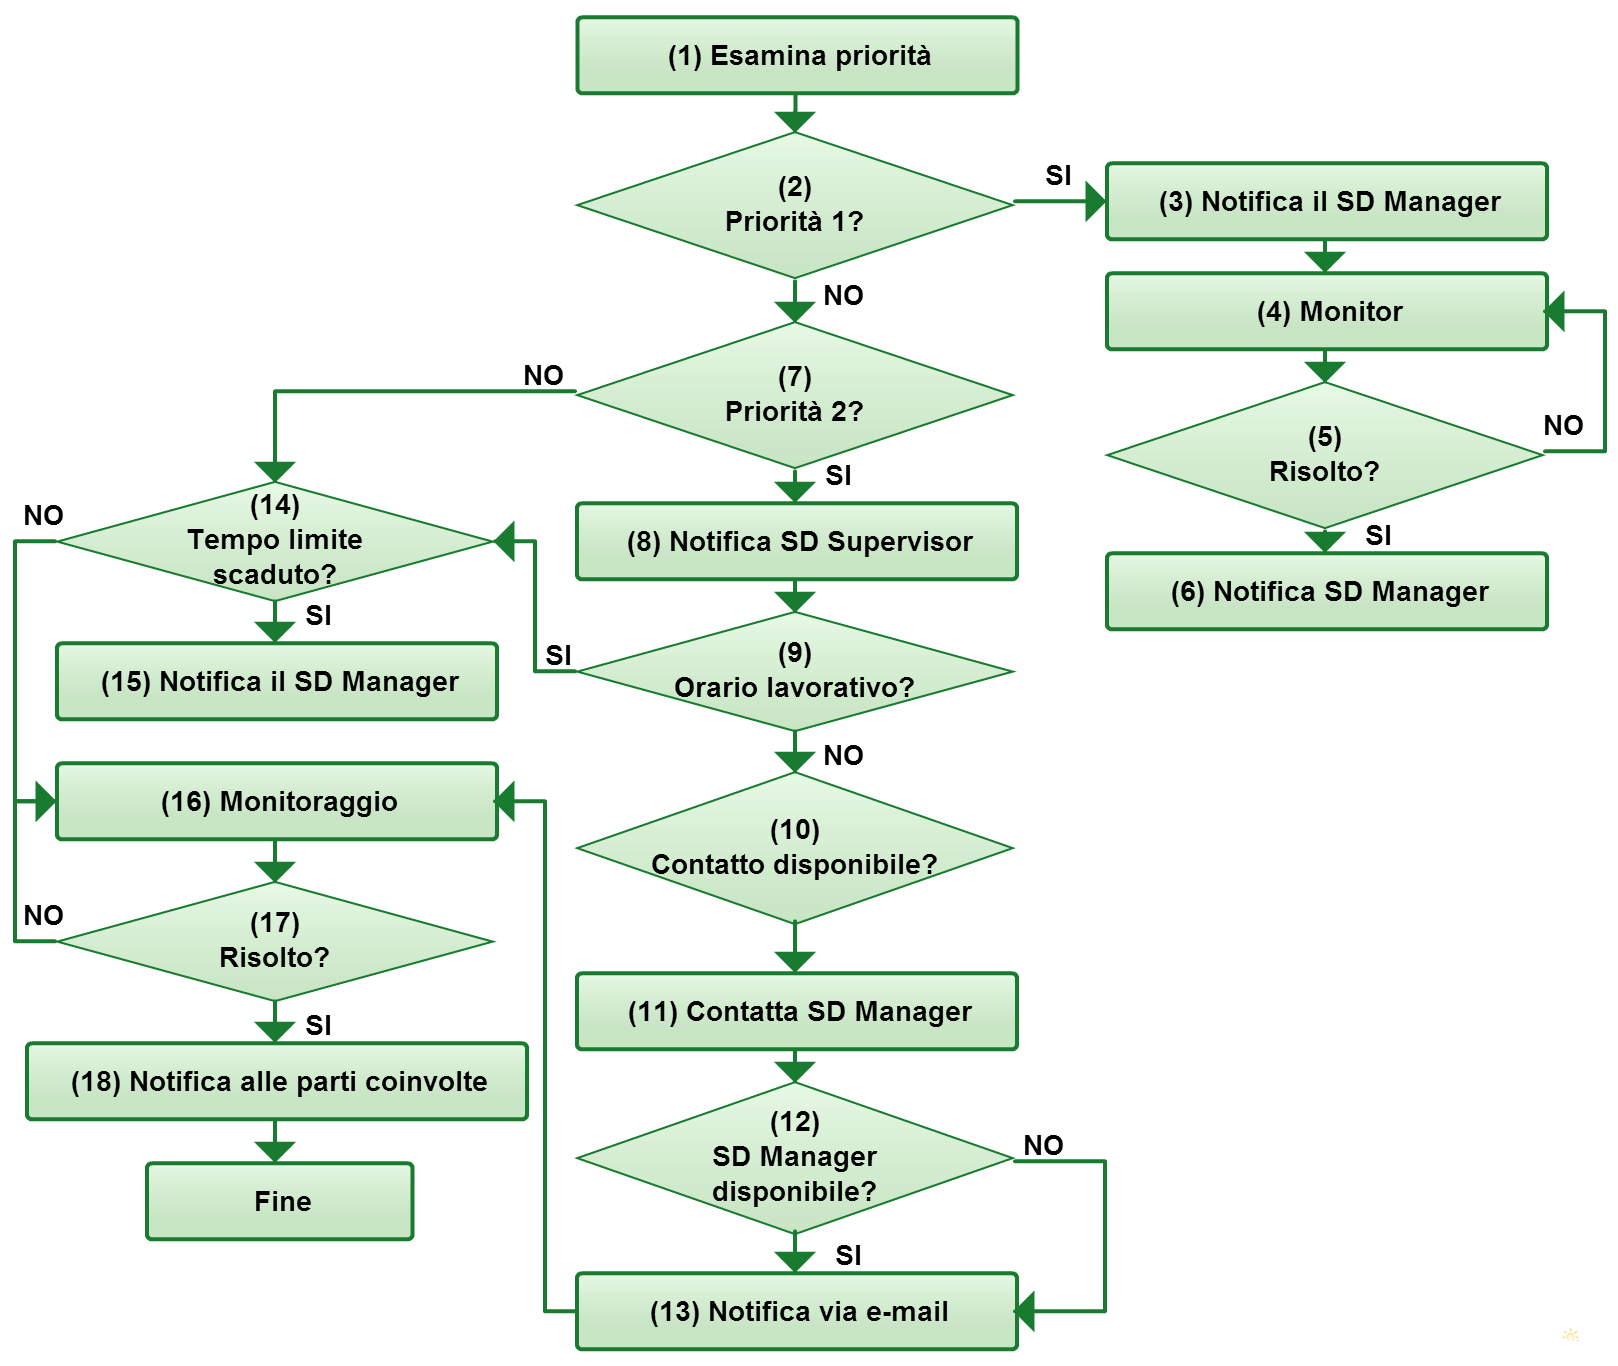
\includegraphics[scale=0.3]{Images/Diagrams/Incident_Management_Escalation_Process.png}
\caption{Attività di \english{escalation}}
\label{im-escalation-activities-img}
\end{figure}

\begin{center}
\begin{longtable}{| p{2cm} | p {10cm} |}
\caption{Elenco attività di escalation}
\label{im-escalation-activities-table}\\
\hline
\multicolumn{1}{| c |}{\textbf{Step}} & \multicolumn{1}{| c |}{\textbf{Descrizione}}\\
\hline
\endfirsthead
\hline
\multicolumn{1}{| c |}{\textbf{Step}} & \multicolumn{1}{| c |}{\textbf{Descrizione}}\\
\hline
\endhead
1 & Esamina tutti gli incidenti ``aperti'' e determina l'azione sulla base della priorità.\\
\hline
2 & Determinare se l'incidente selezionato ha una priorità massima (1 - ALTA).\\
\hline
3 & Se siamo in presenza di un incidente a priorità massima notificare immediatamente al \english{SD Supervisor} corretto ed al \english{SD Manager}. Il \english{SD Manager} deve essere contattato via telefono se non disponibile.\\
\hline
4 & Monitorare lo stato dell'incidente a priorità massima e fornire aggiornamenti almeno ogni 4 ore.\\
\hline
5 & Se l'incidente è stato risolto prosegui al passo 6 altrimenti ritorna la passo 4.\\
\hline
7 & Determinare se l'incidente selezionato ha una priorità media (2 - MEDIA).\\
\hline
8 & Notifica al \english{SD Supervisor} tramite \english{e-mail}.\\
\hline
9 & Determinare se l'incidete è avvenuto in orario di lavoro oppure no. Se avvenuto in orario lavorativo procedi al passo 14.\\
\hline
10 & L'incidente è avvenuto fuori orario lavorativo determinare se la persona di riferimento è raggiungibile. Se raggiungibile notificarla.\\
\hline
11 & Se la persona di riferimento non è raggiungibile notificare il \english{SD Manager}.\\
\hline
12 & Determinare se il \english{SD Manager} è disponibile.\\
\hline
13 & Se disponibile notificarlo verbalmente, altrimenti notificarlo tramite \english{e-mail} e telefono.\\
\hline
14 & Determinare se si è sforato il tempo limite determinato nello \ac{Service-Level-Agreement}.\\
\hline
15 & Se il tempo limite è stato sforato notificare il \english{SD Manager} via \english{e-mail}.\\
\hline
16 & Continuare a monitorare l'incidente.\\
\hline
17 & Determinare se l'incidete è stato risolto. Se non risolto tornare al passo 16 altrimenti proseguire con il 18.\\
\hline
18 & L'incidente è stato risolto notificarlo a tutte le persone che sono state coinvolte nei precedenti passi.\\
\hline
\end{longtable}
\end{center}